
% Somewhere: .map() for recoding

\chapter[Associative arrays in Python (1 of 3)]{\huge\selectfont{Associative
arrays in Python (1 of 3)}}
\label{ch:assocArraysInPython1}

\index{associative array}
\index{Pandas package}
\index{package}
\index{importing (a package)}

Our next trick is to represent associative arrays (review
section~\ref{sec:assocArrays} if you need to) in Python. To do so, we will
use another package, which goes by the adorable name ``Pandas'':

\begin{Verbatim}[fontsize=\small,samepage=true,frame=single,framesep=3mm]
import pandas as pd
\end{Verbatim}

This code should go at the top of your first notebook cell, right under your
``\texttt{import numpy as np}'' line. The two go hand in hand.

\index{table}
\index{NumPy package}
\index{series@\texttt{Series} (Pandas)}
\index{dict@\texttt{dict} (dictionary)}

By the way, just as there were other choices besides NumPy \texttt{ndarray}s to
represent ordinary arrays, there are other choices in Python for associative
arrays. The native Python \texttt{dict} (``dictionary'') is an obvious
candidate. Because this won't work well when the data gets huge, however, and
because using Pandas now will set up our usage of tables nicely in the next
few chapters, we're going to use the Pandas \textbf{Series} data type for our
associative arrays.


\section{The Pandas \texttt{Series}}
\label{sec:creatingSeries}

\index{array!associative}
\index{key-value pair}
\index{series@\texttt{Series} (Pandas)}

A \texttt{Series} is conceptually a set of key-value pairs. The keys are
normally homogeneous, and so are the values, although the keys might be of a
different type than the values. Any of the three atomic types are permissible
for either.

\index{index@index (pl:~indices)}
\index{deep}

Somewhat confusing is that the Pandas package calls the keys ``the
\textbf{index},'' which is an overlap with the term we used for ordinary arrays
(see p.~\ref{arrayIndex}). It's not a total loss, though, since if you think
hard about it, you'll realize that in some sense, \textit{a regular array is
really just an associative array with consecutive integer keys.} Oooo, deep. If
you consider the two halves of Figure~\ref{fig:assocArraysAreArrays}, I think
you'll agree.

\begin{figure}[ht]
\centering
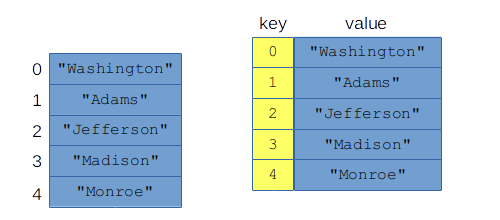
\includegraphics[width=0.9\textwidth]{assocArraysAreArrays.png}
\caption{An ordinary array, and an associative array, that represent the same
information.}
\label{fig:assocArraysAreArrays}
\end{figure}


\subsection{Creating \texttt{Series}es}

Here are a few common ways of creating a Pandas \texttt{Series} object in
memory.

\subsubsection{Way 1: create an empty \texttt{Series}}

Perhaps this first one sounds dumb, but we will indeed have occasion to start
off with an empty \texttt{Series} and then add key/value pairs to it from
there. The code is simple:

\begin{Verbatim}[fontsize=\small,samepage=true,frame=single,framesep=3mm]
my_new_series = pd.Series()
\end{Verbatim}

Voil\`{a}.

\subsubsection{Way 2: \texttt{pd.Series([], index=[])}}

As with NumPy \texttt{ndarrays}, we can explicitly list the values we want in a
new \texttt{Series}. We also have to list the \textbf{index} values (the keys).
The syntax for doing so is:

\label{marvelSeries}
\index{Marvel comics}

\begin{Verbatim}[fontsize=\small,samepage=true,frame=single,framesep=3mm]
alter_egos = pd.Series(['Hulk','Spidey','Iron Man','Thor'],
    index=['Bruce','Peter','Tony','Thor'])
\end{Verbatim}

This creates the \texttt{Series} shown in Figure~\ref{fig:Series}.

\begin{figure}[ht]
\centering
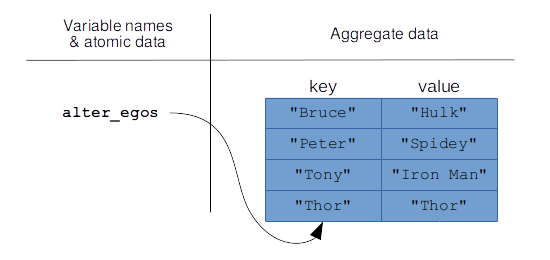
\includegraphics[width=0.8\textwidth]{Series.png}
\caption{A Pandas \texttt{Series} in memory.}
\label{fig:Series}
\end{figure}

\index{boxies (square brackets)}
\index{[]@\texttt{[]} (boxies)}
\index{bananas (parentheses)}
\index{()@\texttt{()} (bananas)}

Be careful to keep all your boxies and bananas straight. Note that both the
keys \textit{and} the values are in their own sets of boxies.

We can print (small) \texttt{Series}es to the screen to inspect their contents:

\begin{Verbatim}[fontsize=\small,samepage=true,frame=single,framesep=3mm]
print(alter_egos)
\end{Verbatim}

\begin{Verbatim}[fontsize=\small,samepage=true,frame=leftline,framesep=5mm,framerule=1mm]
Bruce        Hulk
Peter      Spidey
Tony     Iron Man
Thor         Thor
dtype: object
\end{Verbatim}

\index{type@\texttt{type()}}
\index{dtype@\texttt{.dtype} (NumPy/Pandas)}
and as we did on p.~\pageref{arrayType}, we can inquire as to both the
overarching type of \texttt{alter\_egos} and also to the kind of underlying
data it contains:

\begin{Verbatim}[fontsize=\small,samepage=true,frame=single,framesep=3mm]
print(type(alter_egos))
print(alter_egos.dtype)
\end{Verbatim}

\begin{Verbatim}[fontsize=\small,samepage=true,frame=leftline,framesep=5mm,framerule=1mm]
pandas.core.series.Series
object
\end{Verbatim}

Just as it did on p.~\pageref{dtypeRules}, the ``\texttt{object}'' here is just
a confusing way of saying ``\texttt{str}''. Don't read anything more into it
than that.

\subsubsection{Way 3: ``wrapping'' an array}

\index{dimension}

Associative arrays, and the Pandas \texttt{Series}es we've been using to
implement them, are inherently \textit{one}-dimensional data structures. This
is just like the NumPy arrays we used before. Pandas Serieses also provide a
bunch of features for manipulating, querying, computing, and even graphing
aspects of their content. It's a lot of rich stuff on top of plain-old NumPy.

\index{wrapping}

For this reason, it's common to want to create a \texttt{Series} that just
``wraps'' (or encloses) an underlying NumPy \texttt{ndarray}, and provides all
that rich stuff.

The way to do this is simple:

\begin{Verbatim}[fontsize=\small,samepage=true,frame=single,framesep=3mm]
my_numpy_array = np.array(['Ghost','Pumpkin','Vampire','Witch'])
my_pandas_enhanced_thang = pd.Series(my_numpy_array)
\end{Verbatim}

You can then treat \texttt{my\_pandas\_enhanced\_thang} as an ordinary
aggregate variable which has the more sophisticated operations of next chapter
automatically glommed on to it. The keys (index values) of this thang will
simply be the integers 0 through 3.

\subsubsection{Way 4: \texttt{pd.read\_csv()}}

Finally, there's reading data from a text flie, which as I mentioned back in
section~\ref{np.loadtxt} (p.\pageref{np.loadtxt}) is actually the most common. 
Data typically resides in sources and files external to our programming
environment, and we want to do everything we can to play ball with this open
universe.

The \texttt{pd.read\_csv()} function is a bit awkward since it has several
mandatory arguments if you want to deal with \texttt{Series}es. Here's how it
works. Suppose there were a file called \texttt{disney\_rides.csv} whose
contents looked like this:

\begin{Verbatim}[fontsize=\small,samepage=true,frame=single,framesep=3mm]
Pirates of the Carribean,25
Small World,20
Peter Pan,29
\end{Verbatim}

These are the current expected wait time (in minutes) for each of these Disney
World rides at some point of the day.

To read this into a \texttt{Series} we'd write:

\begin{Verbatim}[fontsize=\small,samepage=true,frame=single,framesep=3mm]
wait_times = pd.read_csv('disney_rides.csv', index_col=0, squeeze=True,
    header=None)
\end{Verbatim}

Most of that junk is just to memorize for now, not to fully understand. If
you're curious, \texttt{index\_col=0} tells Pandas that the first (0th) column
-- namely, the ride names --should be treated as the \texttt{index} for the
\texttt{Series}. The \texttt{header=None} means ``there is no separate header
row at the top of the file, Pandas, so don't try to treat it like one.'' If our
\texttt{.csv} file \textit{did} have a summary row at the top, containing
labels for the two columns, then we'd skip the \texttt{header=None} part.
Finally, ``\texttt{squeeze=True}'' tells Pandas, ``since this is so skinny
anyway -- just two columns -- let's have \texttt{pd.read\_csv()} return us a
\texttt{Series}, rather than a more complex \texttt{DataFrame} object (which is
the subject of a future chapter.)''
